\chapter[Tagish and Tlingit Place Naming Traditions of Southwestern Yukon]{\vspace{-25pt}Tagish and Tlingit Place Naming Traditions of Southwestern Yukon: Evidence of Language Shift}


\sethandle{10125/24845}

% Author last name as it appears in the header
\def\authorlast{Moore}

% change author in three references below to the actual author name so that this name is unique and matches the \label commands just below and at the end of the chapter
\renewcommand{\beginchapter}{\pageref{moore-ch-begin}}
\renewcommand{\finishchapter}{\pageref{moore-ch-end}}
\label{moore-ch-begin}



\thispagestyle{firststyle}

\chapauth{Patrick Moore}
\affiliation{University of British Columbia}

\authortoc{Patrick Moore}


\section{Introduction}
Indigenous place names from the southwestern Yukon reflect a historical shift from the widespread use of Tagish, a northern Dene (Athabaskan) language, to a predominance of Tlingit (a distantly related Na-Dene language). While language shift between indigenous languages has undoubtedly been a common process in many regions of North America, the southwestern Yukon is unusual in that the shift from Tagish to Tlingit occurred relatively recently. Research on indigenous place names has increased in recent years  because of anthropological interest in the cultural conceptualization of place and space, and because of the extensive documentation of land use related to indigenous land claims. Most of this work has focused on the place names of particular groups and regions, but some studies have also examined the contested nature of place naming in relation to colonialism, competing languages, language shift, and the displacement of indigenous peoples (Young 2001; Berg and Vuolteenaho 2009; Hercus, Hodges and Simpson 2009; Weinreich 2011). This study focuses specifically on the evidence that Tagish and Tlingit place names provide concerning the history of Tagish and Tlingit interaction and language shift in the southwest Yukon. This region is unusual in that a large number of place names have been recorded in both languages providing an opportunity to examine the processes of language change and evidence that Tagish was formerly the dominant language in this region but was gradually replaced by Tlingit.  While intermarriage between the coastal Tlingit and the adjacent Tagish of the Yukon interior was likely common even before the arrival of Europeans, Tlingits' control of the fur trade between the Pacific coast and the southern Yukon greatly increased their prestige and economic influence in the nineteenth century. Tagish adopted the Tlingit moiety and clan systems, and many adopted Tlingit personal names. According to Tagish speaker Daisy Smith (personal communication) by the late 1800s the remaining speakers of Tagish were all bilingual in Tlingit. The place names that form the basis of this study were originally recorded in both Tlingit and Tagish and identified on a map of the region by Angela Sidney and anthropologist Julie Cruikshank (Sidney 1980). Jeff Leer of the Alaska Native Language Center provided the Tlingit transcriptions of Sidney’s place names. For this article the transcriptions for the Tagish place names have been updated to a contemporary Tagish orthography developed by linguists working with the Yukon Native Language Centre\footnote{The symbols used in the Tagish alphabet are described on the Yukon Native Language Centre website at \url{http://www.ynlc.ca/tagish.shtml\#alphabet}}  and the translations and transcriptions of the Tlingit place names were rechecked with Bessie Cooley, a Tlingit speaker from Teslin, Yukon.\footnote{The Tlingit orthography used here is the same as the system developed by Gillian Story and Constance Naish and described on the Sealaska Heritage Foundation website at \url{http://www.sealaskaheritage.org/sites/defaults/files/tlingit_alphabet.swf}. The Naish/Story orthography is used in this article because it was the writing system used by Sydney and Cruikshank in their 1980 publication and because it remains in popular use. An alternative orthography for Tlingit was later developed by Jeff Leer and popularized by the Yukon Native Language Centre in their publications.}  The numbering of the examples is the same as in Sidney 1980, which is the source of all the place names in this chapter unless otherwise noted.

By the early twentieth century Tlingit was the predominant indigenous language in the Carcross and Tagish regions of southwestern Yukon, although a few families continued to speak Tagish as well as Tlingit and to use it with their children as well. The area also experienced an influx of English speakers after 1898 as it was situated on the main route to the Klondike Gold Rush. Tagish children who grew up in the early 1900s, among them Daisy Smith, Johnny Johns, and Angela Sidney, became some of the last fluent speakers of Tagish, and as adults worked with linguists and anthropologists to document their languages and cultures in the last decades of the twentieth century. Lucy Wren (personal communication), one of the last people to acquire first-language fluency in the language, recalled that her parents spoke to her only in Tlingit, but that Tagish was still commonly used between the adults in her home, and she was able to learn the language even though her parents avoided using it with her.	A small number of anthropologists and linguists documented Tagish language and culture the last half of the twentieth century. In the 1960s, anthropologist Catherine McClellan documented Tagish cultural practices, beliefs and stories (McClellan 1975, 2007). Later, linguists and anthropologists associated with the Yukon Native Languages Project, which became the Yukon Native Languages Centre, documented the Tagish language and Tagish traditions. Julie Cruikshank worked extensively with Mrs. Angela Sidney, a fluent speaker of both Tagish and Tlingit to document stories (Cruikshank 1989, 1992), genealogies (Sidney 1983), and place names (Sidney 1980). Victor Golla, Jeff Leer, John Ritter, and Patrick Moore worked with Tagish speakers, principally Angela Sidney and Lucy Wren, to record the language in the form of field notes, basic language lessons (Wren 2005-2007), and as audio and video recordings. Most of the Tagish language documentation is housed at the Yukon Native Language Centre, and a description of the Tagish alphabet, audio lessons, and audio storybooks are available from the Centre. A large number of Tagish recordings and written materials are also housed at the Alaska Native Language Archive of the Alaska Native Language Center and can be accessed online for non-commercial use.

\section{General Evidence of Length of Occupancy and Extent of Later Interaction}

The evidence from Tagish and Tlingit place names is consistent with the view that the area where Tlingit was spoken expanded, first northward within coastal Alaska and then into the interior.  Jeff Leer (1979) has argued for a northward expansion of Tlingit, since conservative features, such as constricted vowels, are found only in the southern Tongass dialect of Tlingit. In contrast, the Tagish language may have had a long history of development in the area where it was spoken in recent times. Based on a comparative study of terms for \textit{stream} in Dene (Athabaskan) languages, James Kari (1996a, 1996b) has argued that the historic Dene homeland was in the region where contemporary Dene languages use [tu·] for \textit{stream}, an area that includes the region where Tagish was historically spoken. This conservative word for \textit{stream} is evident in many of the place names that Cruikshank recorded with Angela Sidney (1980).\\

 Examples of Tagish place names with [tu·] for ‘stream’:
\begin{exe}

\exi{4.}	McClintock River
\sn Gēs Tū’è’ (Tagish)		king salmon river
\sn T’ahéeni (Tlingit) 		king salmon river
\exi{26.} 	Squanga Creek
\sn 	Dèsgwą̄gè Tū’è’ (Tagish)	Squanga whitefish creek
\sn 	Dasgwaanga Héeni (Tlingit)	Squanga whitefish creek
\end{exe}

Sidney learned Tlingit and Tagish as first languages and was able to provide terms in both for 68\% of the 130 locations. She identified 14\% of the places with only a Tagish name and nearly the same percentage, 18\%, with only Tlingit names. Some of the place names are composed of words from both languages, which indicates the extent of Tagish-Tlingit bilingualism, borrowing, and code-switching.\\

Examples of place names composed from both Tagish and Tlingit terms:
\begin{exe}
\exi{19.}	The single peak separated from Sinwaa, adjacent to the Tagish Road and the
turn-off from the Alaska Highway to Atlin, B.C.
	\sn Shgáa	T’ōh	 (Tlingit then Tagish)	Sidney says that shgáa is the Tlingit name of an
unidentified bird. Cooley was unfamiliar with the word.
The word is almost certainly Tlingit in any case since the sh-g syllable onset violates Tagish but not Tlingit phonological constraints.
T’ōh is Tagish for nest
\exi{55.} 	Tagish Hill
\sn Tā̀gish Tóoli	 (Tagish then Tlingit) Tā̀gish is the Tagish name for the Tagish narrows
	\sn		Tóoli is Tlingit for grassy hill
\exi{80.} Head of Tagish Narrows
\sn Tā̀gish Sháak	 (Tagish then Tlingit) Tā̀gish is the Tagish name for the Tagish narrows
\sn				Sháak is Tlingit for \textit{headwaters}
\end{exe}


The map in Figure~\ref{moore-map} indicates the location of the Tagish and Tlingit named places that are cited in this article. The reference numbers for these places on the map and in the article are the same as used in Sidney’s (1980) book and accompanying map.

\begin{figure}[h]
\centering
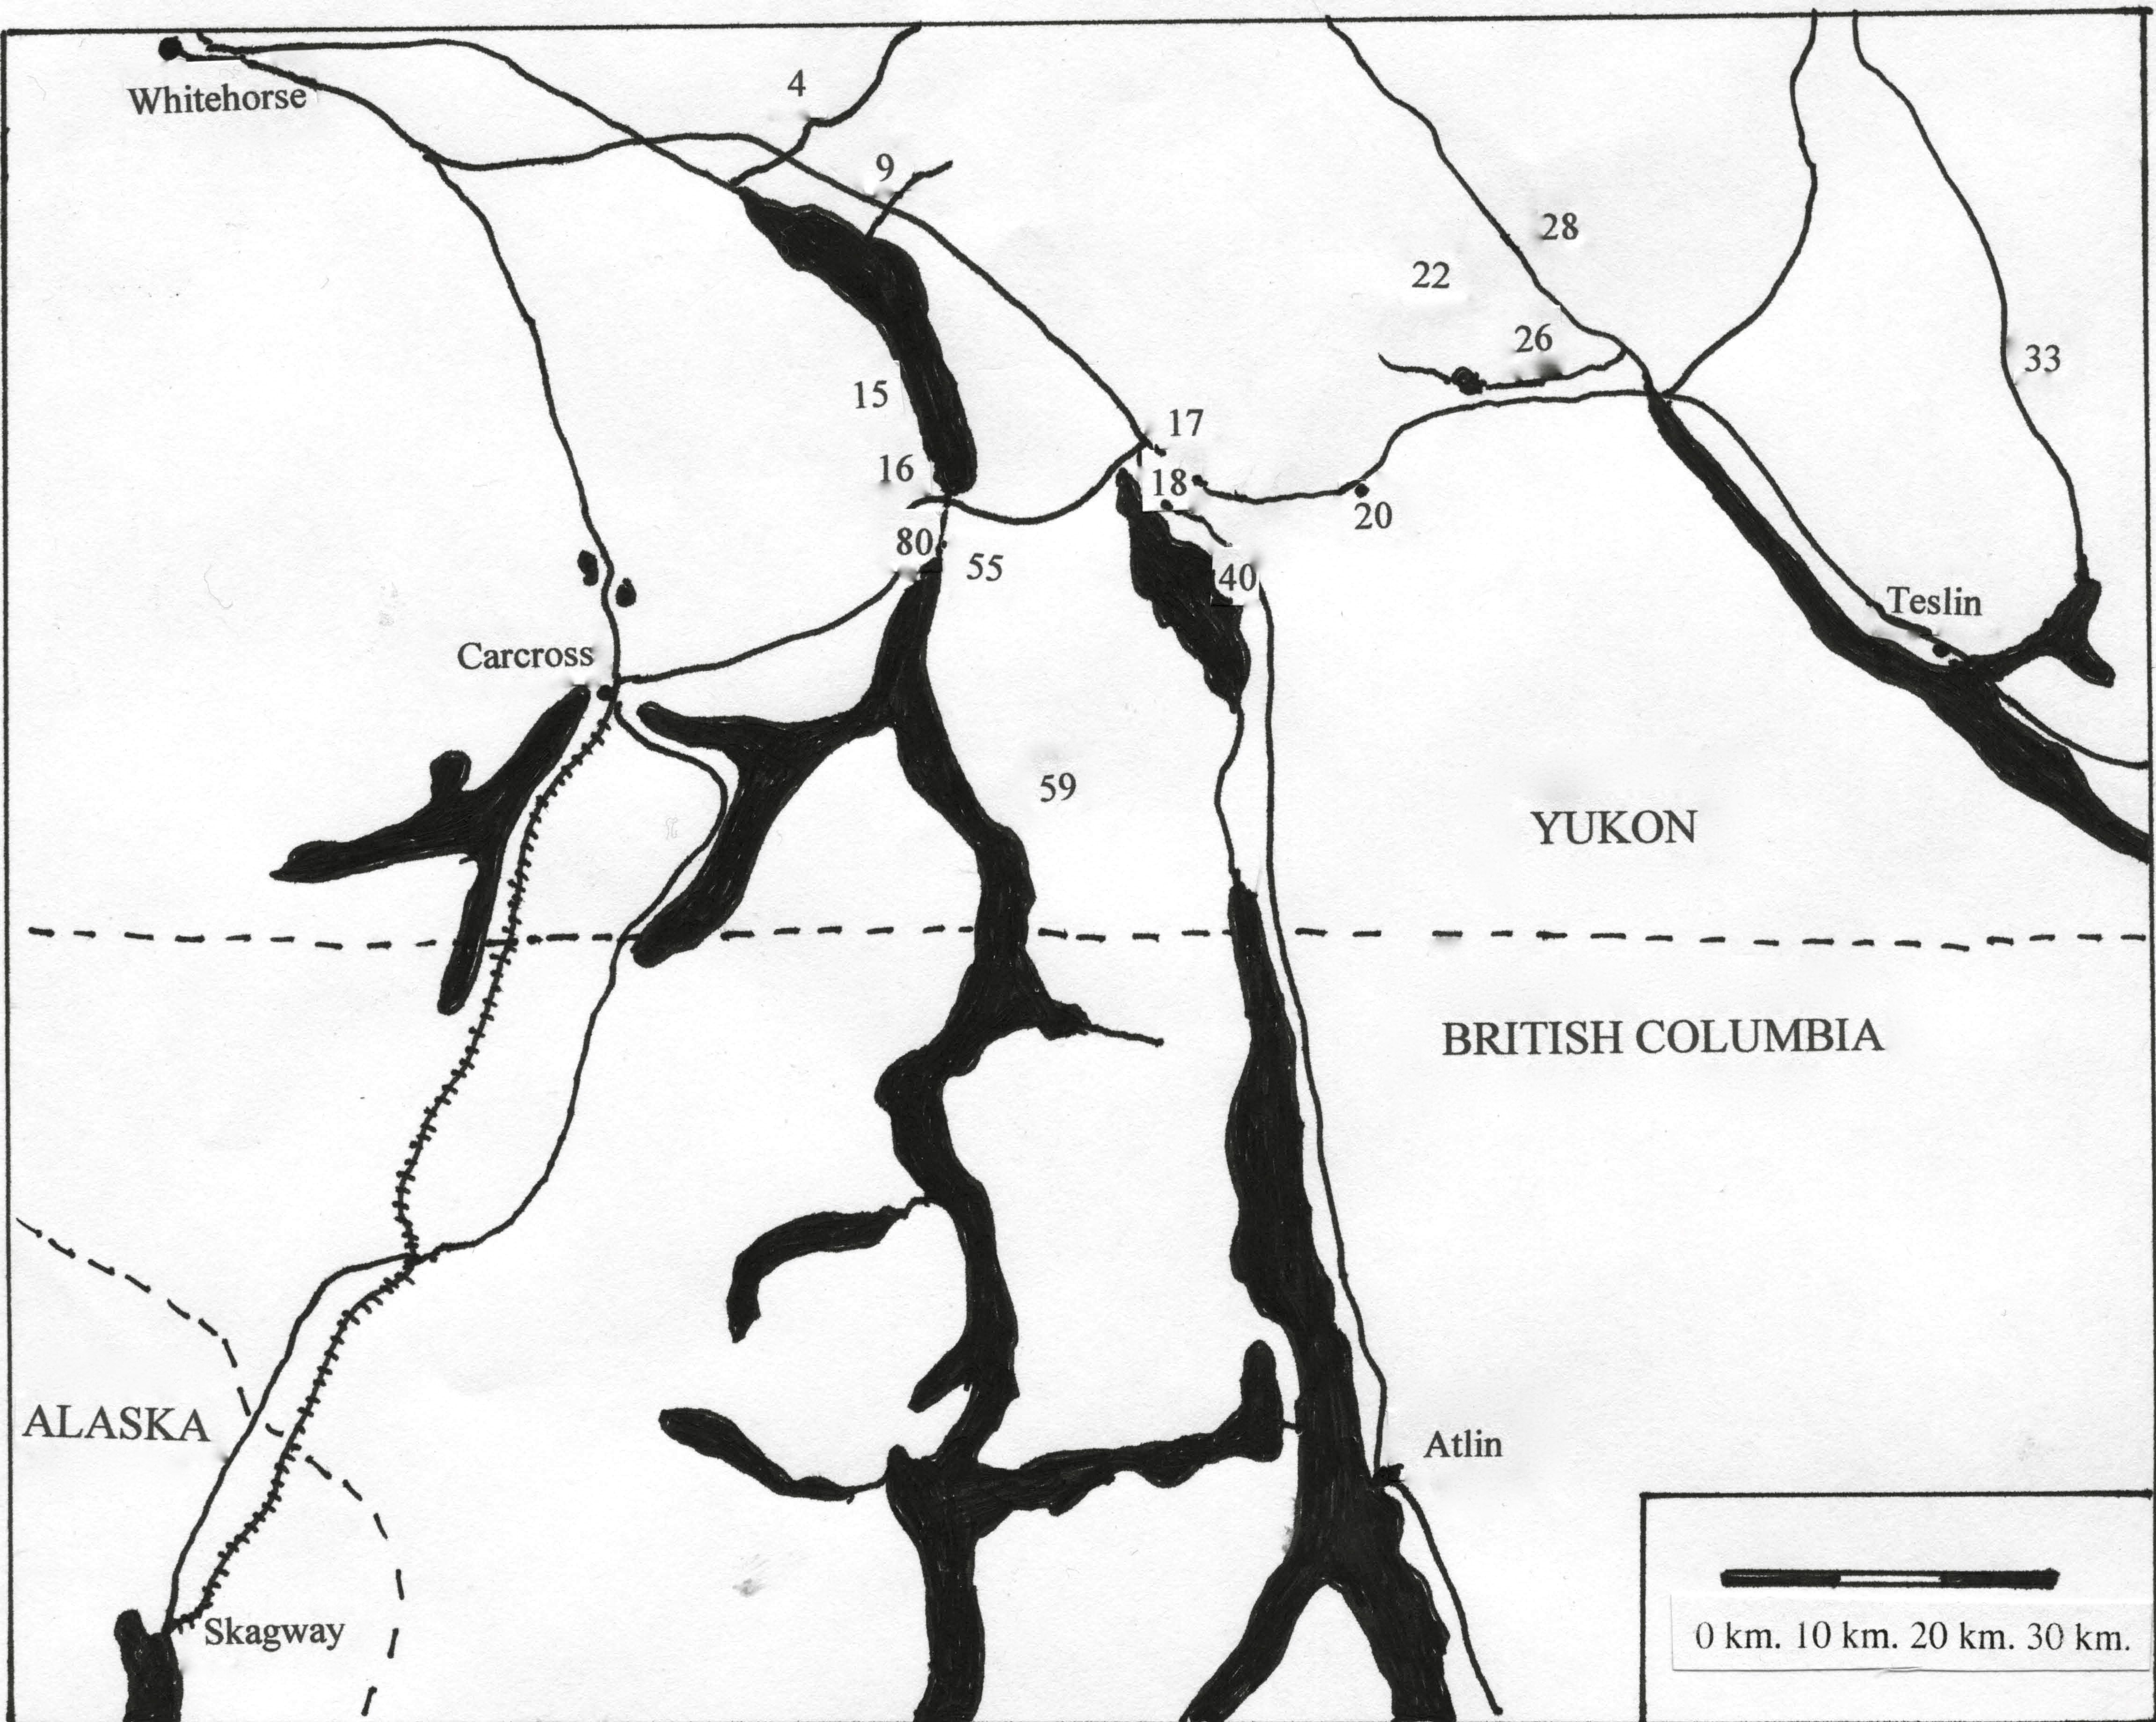
\includegraphics[width=0.9\textwidth]{figures/moore-fig1}
\caption{Locations of Selected Tagish and Tlingit Named Places}\label{moore-map}
\end{figure}

\section{Place Name Evidence of Language Shift from Tagish to Tlingit}
While all of the Tagish speakers were also fluent in Tlingit by the late 1800s, in the course of changing Tagish place names into Tlingit names they often modified the Tagish originals in ways that point to both Tagish as the source language and to the coastal connections of Tlingit. Some Tlingit place names (\textit{Sinwaa}, \textit{Nisaleen}) or parts of place names (\textit{Deisleen}) are not meaningful in Tlingit because they are based on the sound of the Tagish name. Some parts of Tagish names were omitted as they were translated into Tlingit, and in at least one case a Tlingit place name (\textit{Sheix’w X’aayi}) uses a term for a tree found in coastal southeast Alaska in a new sense in the interior.

While the Tlingit place names recorded by Angela Sidney are often composed of the same meaningful elements as the Tagish place name, in some cases, such as 18 below, the Tlingit term is based on the Tagish words modified to conform to the Tlingit sound system. In this case the Tlingit place name is not composed of elements that are meaningful in Tlingit.

Bessie Cooley (personal communication) says Sinwaa is also the name of a mountain near the Taku River (see also Nyman and Leer 1993 for confirmation of this term). It is possible that the Tlingit name for that mountain was also based on an Athabaskan name. Names referring to limestone, “grey rock,” may be common in Dene languages of this region. There is a Southern Tutchone name of the same form, \textit{Sima} (grey rock) which is the name of Golden Horn Mountain south of Whitehorse. The Tagish term from Lucy Wren is from the Tagish Literacy Workshop held in 1994 (Moore 1994: 15); the Tlingit term doesn’t mean limestone and is likely based on the sound of the Tagish word as it is only meaningful as a place name.\\

Tlingit place names based on the sound of the Tagish name:
\begin{exe}
\exi{18.} The mountain southeast of Jakes Corner between the Alaska Highway and the Atlin Road, excluding the first mountain peak.
	\sn Tsambā’a (Tagish, Angela Sidney)	`grey ridge'
	\sn Tsē Mbā (Tagish, Lucy Wren)		`grey rock'
	\sn Sinwaa (Tlingit from Athabaskan)
\exi{28.} Teslin River
	\sn Dèdèslīnī̀  (Tagish)			`water running off'
	\sn Deisleen Íxde Naadaayí		`Teslin running downstream'
\exi{33.} Nisutlin River
	\sn Dèslī́nī́ (Tagish)			(flowing [water?])
	\sn Nisaleen or Nilaseen (Tlingit)		(probably from Athabaskan)
\end{exe}



Tlingit speaker Bessie Cooley suggested ‘sneaks’ as a meaning for the Tlingit term Nisaleen, but it appears to be based on a Tagish word that includes the stem –līn, used in reference to flowing water, as in 28. The stem for “flowing water” may be commonly used in Dene (Athabaskan) place names since it also appears in other well-known names such as Deline (“where waters flow”) the North Slavey (and official English) name for the village at the headwaters of the Great Bear River on Great Bear Lake, Northwest Territories. The Tagish term in 33 is similar to the Tlingit (and English) terms for the village of Teslin, Yukon. The Tlingit (and English) terms for Nisutlin are likely based on a related Athabaskan word that had slightly different prefixes.
In other cases, such as 9 below, Sidney provided a Tlingit translation but indicated that the Tlingit place name wasn’t actually used to identify that location, and that everyone continued to use the Tagish term. The meaning of the Tlingit translation that Sydney provided for 9 below is unclear since Cooley was not familiar with the Tlingit term Keshuwaa (héeni means ‘stream’). Keshuwaa doesn’t mean ‘grayling’ which is t’áse or t’ási in interior Tlingit (likely from Athabaskan).\\

Tlingit translation not actually used as a place name designation:
\begin{exe}
	\exi{9.} 	Grayling Creek
	\sn T’àse Mbèt (Tagish)		`grayling food'
	\sn *Keshuwaa Héeni (Tlingit)	(*The Tlingit translation is not used.)
\end{exe}

At least one of the Tlingit terms that Sidney used in place names, the term for ‘red alder’ sheix’w in 15 below, has a different meaning than it would on the coast and reflects the extension of meanings in a new biotic zone. There are no red alder in the interior, the coastal Tlingit term is used by Tlingit in the interior as the nearest equivalent to red willow. Since the Tagish remained in the same biotic region, this sort of semantic shifts is not evident in Tagish place names.\\

Coastal Tlingit term given a new meaning in the Yukon interior:
\begin{exe}
\exi{15.} Point on the west Side of Marsh Lake
	\sn K’àye Desdel Nī (Tagish)	red willow point
\sn Sheix’w X’aayi (Tlingit)	red alder point
\end{exe}
\noindent
In other cases the Tagish name was simplified when it was translated into Tlingit by leaving out part of the Tagish place name.\\

Tagish place names that are simplified in Tlingit:
\begin{exe}
\exi{16.} A point on the west side of Marsh Lake, near Tagish Bridge
	\sn K’àlā Nī (Tagish)		`willow branches point'
	\sn K’ày’ lā Nī (Tagish)		`willow branches point'
	\sn Ch’áal’ X’aayi (Tlingit)		`willow point'
\exi{17.}  The mountain northeast of Jake’s corner, just north of the Alaska Highway
	\sn Tl’o K’ā̀’ Dzełè’	(Tagish)	`grass blade mountain
	\sn Chookanshaa (Tlingit)		`grass mountain
\exi{40.} Point of land on Little Atlin Lake, just north of the narrows
	\sn Mbesh Te’èts’et Nī (Tagish)	`where a knife fell into the water point
	\sn Lítaa Héent Uwaxixi (Tlingit)	`where a knife fell into the water
\exi{59.} Western extension of Jubilee Mountain
	\sn Kā̀’ Dḕtl’ōni Dzełè’ (Tagish)	`where arrows are tied in a bundle mountain'
	\sn Chooneit Shaayí  (Tlingit)	`arrow mountain' (translation from Athabaskan)
\end{exe}

The Tlingit place name Kaa  Léelk’u Shakanóox’u (below) may be a literal translation of the Tagish terms that loses the non-literal meaning of the Tagish original. In the case below the Tagish word for ling cod fish Kwachų̄ literally means “someone’s grandmother,” and when translated literally in Tlingit it loses the reference to the fish that live in the adjacent lake.\\

Place names that lose their non-literal meaning in translation to Tlingit:
\begin{exe}\exi{22.} “Streak Mountain”, north of Squanga Lake.
	\sn Kwachų̄ Tsī̀ts’enè’ (Tagish)	`ling cod skull'
(literally someone’s grandmother’s skull)
	\sn Kaa  Léelk’u Shakanóox’u (Tlingit)	`one’s grandmother’s skull'
\end{exe}

In both Tagish and Kaska, the names of specific fish or the generic word for fish may be used instead of the word for lake. According to Jeff Leer (personal communication) this place naming convention is not used in coastal Tlingit, so its use in interior Tlingit is evidence of the adoption of Tagish place naming practices as terms were translated into Tlingit. Bessie Cooley cited examples of interior Tlingit place names that use \textit{xáadi} (fish) to identify a lake, including \textit{Kaa Léelk’u Xáadi} (somebody’s grandparent [ling cod] fish), a lake near the south end of Teslin Lake, Yukon and X’aaa Xáadi (red fish), a lake near Teslin, Yukon. Examples from Kaska include \textit{Tets’egelūgé’} (up the hill fish), Watson Lake, 128° 47' W, 60° 08' N; \textit{Dzǭą̄lūgé’} (small bird fish), Little Bird Slough, 131°54' W, 62° 02' N; \textit{Bédelūgé’} (food fish),  a lake that is one of the sources of Blind Creek, 132°46' W, 62° 13' N, \textit{Eyānlūé’} (downstream people fish), No English name, 132° 01'W, 62° 08° N; \textit{Kūk’éhlūgé’} (next behind fish), No English name, 132° 31' W. 62° 31' W; Tāgeslūgé’ (middle fish), No English name, 132° 20' W, 62° 09' N; \textit{Tédāgīlūgé’} (up on top fish) No English name, 132° 44' W, 62° 04' N (Kaska Tribal Council 1997). Interestingly, most of the Kaska names that use \textit{lūge} or \textit{lūe} ‘fish’ as a designation for lakes (all the examples except \textit{Tets’egelūgé’}, which is in the Watson Lake area) are in the northern part of Kaska territory near Ross River, where there were formerly many speakers of Tagish.  In example 20 below the Tagish place name uses \textit{tā̀słeyī̀ }(pike fish) to designate the lake, while the Tlingit place name uses \textit{áayi} (lake).\\

Tagish place name using a fish name instead of ‘lake’:
\begin{exe}
\exi{20.} Squan Lake half way between Jake’s Corner and Squanga Lake. (Skwáan is a Tlingit personal name belonging to the Deisheetaan Clan. The lake may have been named for Joe Squan, or for someone else who held this name).
	\sn Skwān Tā̀słéyī 	(Tagish)	`Squan’s Pikefish'
	\sn Skwáan Áayi (Tlingit)		`Squan’s Lake'
\end{exe}



\section{Conclusion}
The Tagish and Tlingit place names recorded by Angela Sidney (1980) with Julie Cruikshank provide important evidence of both language shift from Tagish to Tlingit in this region of southwest Yukon, and an indication that most Tagish were fully bilingual in Tlingit. Most of the Tlingit place names Sidney recorded (68\%) are exact translations of the Tagish names (calques). There are also a number of place names that incorporate words from both languages, demonstrating that code switching and the use of loan words were common features associated with bilingualism. While most of the Tlingit place names are exact translations of the Tagish terms, the terms that differ provide evidence that the Tagish place names were in use prior to widespread language shift to Tlingit. The processes of simplification, basing Tlingit terms on the sound of Tagish terms, creating translated terms that lose their non-literal sense, adopting or failing to adopt different generic conventions (the use of “fish” for “lake”), and giving Tlingit terms a new semantic sense appropriate to their use in a new biotic zone are all processes that might be expected as a result of the expanded use of Tlingit. In addition to providing detailed information about traditional land and resource use, Sidney’s and Cruikshank’s documentation of the Tagish and Tlingit place names for 130 locations in southwestern Yukon also reveals much about the nature of Tagish and Tlingit bilingualism and local processes of language shift.




%%%% REFERENCES %%%%%%%%%%%%%%%
\refheading

\begin{hang}

Berg, Lawrence \& Jani Vuolteenaho. 2009.	\textit{Critical Toponymies: The Contested Politics of Place Naming}. Farnham, England, Burlington, Vermont: Ashgate.

Cruikshank, Julie. 1990. \textit{Life Lived Like a Story: Life Stories of Three Yukon Native Elders}. Vancouver: University of British Columbia Press.

Cruikshank, Julie. 1998. \textit{The Social Life of Stories: Narrative and Knowledge in the Yukon Territory}. Lincoln: University of Nebraska Press.

Hercus, Luise, Flavia Hodges \& Jane Simpson (eds.). 2009. \textit{Land is a Map: Placenames of Indigenous Origins in Australia}. Canberra: ANU Press.

Leer, Jeff. 1979. \textit{Proto-Athabaskan Verb Stem Variation Part One: Phonology}. Fairbanks: Alaska Native Language Centre, University of Alaska Fairbanks.

Kari, James. 1996a.	A Preliminary View of Hydronymic Districts in Northern Athabaskan Prehistory. \textit{Names} 44(4). 253-271.

Kari, James. 1996b. Names as Signs: The Distribution of ‘Stream’ and ‘Mountain’ in Alaska Athabaskan Languages. In Eloise Jelinek, Sally Midgette, Keren Rice \& Leslie Saxon (eds.), \textit{Athabaskan Language Studies: Essays in Honour of Robert Young}, 243-268. Albuquerque: University of New Mexico Press.

Kaska Tribal Council
1997	Guzāgi Kūgé’: Our Language Book: Nouns, Kaska, Mountain Slavey and Sekani. Whitehorse: Kaska Tribal Council.

McClellan, Catherine. 1975.	\textit{My Old People Say: An Ethnographic Survey of Southern Yukon Territory, Parts 1 and 2}. Ottawa National Museum of Man.

McClellan, Catherine. 2007.	\textit{My Old People’s Stories: A Legacy for Yukon First Nations}. Whitehorse: Yukon Tourism and Culture.

Moore, Patrick. 1994. \textit{Tagish Literacy Workshop}. Whitehorse, Yukon: Carcross Tagish First Nation.

Nyman, Elizabeth \& Jeff Leer. 1993 	\textit{Gágiwdułàt: Brought Forth to Reconfirm: the Legacy of a Taku River Tlingit Clan}. Whitehorse: Yukon Native Language Centre, Fairbanks: Alaska Native Language Center.

Sidney, Angela. 1980. \textit{Place Names of the Tagish Region, Southern Yukon}. Whitehorse: Council for Yukon Indians.

Sidney, Angela. 1983. \textit{Haa Shagóon: Our Family History}. Whitehorse, Yukon: Council for Yukon Indians.

Weinreich, Uriel. 2011. \textit{Languages in Contact: French, German and Romansch in Twentieth-Century Switzerland}. Amsterdam, Philadelphia: John Benjamins.

Wren, Lucy. n.d. \textit{Tagish Language Lessons}. Victoria British Columbia: FirstVoices, First Peoples Cultural Heritage Foundation. \url{http://www.firstvoices.com/explore/FV/sections/Data/Yukon/Tagish/Tagish}, accessed January 25, 2019.

Wren, Lucy. 2005-2007.	\textit{Tagish Language Lessons}. Whitehorse: Yukon Native Language Centre.
\url{http://www.ynlc.ca/tagish.shtml\#lessons}
accessed January 25, 2019.

Young, Kee How. 2001. The Politics and Aesthetics of Placenames in Sarawak. \textit{Anthropological Quarterly} 80(1). 65-91.

\end{hang}

\orcidfooter{Patrick Moore}{}{}

\label{moore-ch-end}
